
\documentclass[11pt]{article}

% My packages
\usepackage{graphicx}
\usepackage[tight,footnotesize]{subfigure}
\usepackage[cmex10]{amsmath}
\usepackage{amsfonts}
\usepackage{amssymb}
\usepackage{textcomp}
\usepackage{bbm}        % Needed for the indicator function
\usepackage{algorithm}
\usepackage{algorithmic}
\usepackage{booktabs}   % Schoener tables!
\usepackage{url}
\usepackage{subfigure}
% \usepackage{robinmath}

\usepackage[english]{babel}

\usepackage[style=footnote-dw]{biblatex}
% Package biblatex: '\bibliography' must be given in preamble.
\bibliography{bibliography}

% these are the package necessary to implement the required layout for the conference
\usepackage[left=2.54cm,right=2.54cm,top=1.25cm,bottom=2.54cm]{geometry}
\usepackage{titlesec}
\usepackage[scaled]{uarial}

\titleformat{\section}{\Large\usefont{T1}{phv}{b}{n}}{\thesection}{1em}{}

\newcommand*{\TitleFont}{%
  \Large\usefont{T1}{phv}{b}{n}%
    \selectfont}

\newcommand*{\AuthorFont}{%
  \normalsize\usefont{T1}{\rmdefault}{m}{n}%
    \selectfont}

\usepackage{times}



% *** Do not adjust lengths that control margins, column widths, etc. ***
% *** Do not use packages that alter fonts (such as pslatex).         ***
% There should be no need to do such things with IEEEtran.cls V1.6 and later.
% (Unless specifically asked to do so by the journal or conference you plan
% to submit to, of course. )


% correct bad hyphenation here
\hyphenation{op-tical net-works semi-conduc-tor}


\begin{document}
%
% paper title
% can use linebreaks \\ within to get better formatting as desired
\title{\TitleFont Crowd-sourced citizen-driven mobile sensing of radiation}


% author names and affiliations
% use a multiple column layout for up to two different
% affiliations

\author{
  \AuthorFont Robin Scheibler, Christopher Wang, Kalin Kozhuharov, Joe Moross, Pieter Franken, \\
  \AuthorFont Tomoyuki Furutani, and Keisuke Uehara \\
  \AuthorFont Keio Research Institute at SFC, Fujisawa, Kanagawa, Japan
}

% no date in the title
\date{}

% make the title area
\maketitle

% remove page number
\thispagestyle{empty}
\pagestyle{empty}

\section*{Abstract}
\label{sec:abstract}
% no \IEEEPARstart

Amid the recent triple meltdown at Fukushima Dai-ichi plant that followed the Great Tohoku Earthquake and Tsunami, radiation fears dormant since Chernobyl were suddenly awaken.
During the early time of the crisis, all the radiation measurements were done by the Ministry of Education, Culture, Sports, Science and Technology (MEXT) as 
well as the operator of the plant, Tokyo Electric Power Company (TEPCO), both having a vested interest in controlling the value of the measurements published.
In addition to that the measurement data was published in a format unsuitable for machine reading and the data was not released free of rights,
making it difficult to use for academic purposes.

Another drawback of this data set is that it is collected by fixed sensors. Fixed sensors offer a really good temporal resolution, making it suitable for
early detection of new radioactive pollutant release detection. However, it has a very poor spatial resolution. Since radioactive plume fall-out is notoriously
spurious because of the airborne travel mode [REF], a high spatial resolution is needed in order to precisely assess the contamination at the level of houses.
This is necessary for multiple reasons, including, first of all, to assess the health hazard and plan evacuation areas accordingly, plan efficiently decontamination
work, identify areas still suitable for farming.

To add to the challenge, the Geiger counters and other measurement devices were quickly sold-out, making it necessary to efficiently use the few devices that
were available at the time.

Recently, mobile sensor networks have emerged as a very efficient way to cover large areas in detail using much fewer sensors than a fixed network, at the expense
of time resolution [REF]. In the case of radiation contamination with Cesium 134 and Cesium 137, with respective half-lives of 2 and 30 years, this is a fair trade-off.

We present the design of a mobile radiation sensor network for independent citizen monitoring and cartography of radioactive contamination.
Even if mobile radiation measurement is not new [REF], historically radiation measurements has had a high entry barrier for technical and political reasons.
We want to show how the tremendous advances in information technology, and the Internet in particular, have been a game changer in this field. In addition, we show how
open-source software and hardware paradigm allowed for extremely fast development and deployment of the sensor network.

Because of the citizen-driven and privately funded nature of the project, the design needs to be very cost-efficient. Off-the-shelf hardware was used to create
a first system composed of a Geiger counter, a commercial GPS USB dongle, a micro-controller board and netbook. The audio output of the Geiger counter
was plugged to an Arduino board outputing the count-per-minute (CPM) every five seconds over serial port. The netbook then aggregates the geographic location
obtained from the GPS and the radiation count and writes it to a file every five seconds. A diagram of the system is given in Fig. [FIG].

The Geiger counter chosen is the Inspector Alert [REF] that uses an industry standard [REF] LND73... two-inch pancake tube [REF].
The Geiger counter, the Arduino board and the GPS are housed in a waterproof box.
This box is fixed to the side of a car using a simple system of straps that can be easily fixed on any car by winding up a window on the strap as shown in Fig. [FIG].
Suction cups on the back of the box then ensure that the box is firmly attached and do not vibrate, even driving at higher speed on the highway.

In order to cover rapidly vast areas, the driving of the sensors was crowd sourced to volunteers based in the contaminated areas in Tohoku.
The volunteers then drove the sensors during their daily activities. Once a volunteer would finish to cover her own neighborhood or city, the sensor
could be dispatched to another volunteer living in a different area.

After collection, the data file produced is manually (as of now) uploaded to an online database. From this database, comprehensive maps as shown in Fig. [FIG] 
are created and released. The raw data is also released without copyright and in machine readable format, allowing it to be easily reused for further research.


\section*{Motivation}
\label{sec:motivation}

Due to the recent triple meltdown at the Fukushima Dai-ichi plant in Japan, dormant fears about radiation have been awaken.
Radiation is present throughout nature due to cosmic rays and the radioactive decay of naturally occuring isotopes such as Uranium or Thorium.
Despite being discovered in the early 20\textsuperscript{th} century [TBA], the health effect of radiation was only brutally revealed to the public at
large after the bombing of Hiroshima and Nagasaki during World War II [TBA]. This was followed by extensive atmospheric nuclear testing throughout the 50's and 60's.
Atmospheric testing was subsequently banned after the health effect of lower doses of radiation became apparent on down-winders living close to
nuclear test site in the USA [TBA].

Mobile survey of radiation in Chernobyl\cite{arvela1990mobile}.

\section*{Results}
\label{sec:results}

Here give some results.

\begin{figure}[ht]
\centering
\subfigure[Global map of collected data for the Fukushima prefecture.
            Each square is color coded according to the average dose
            rate in the area covered.]{
  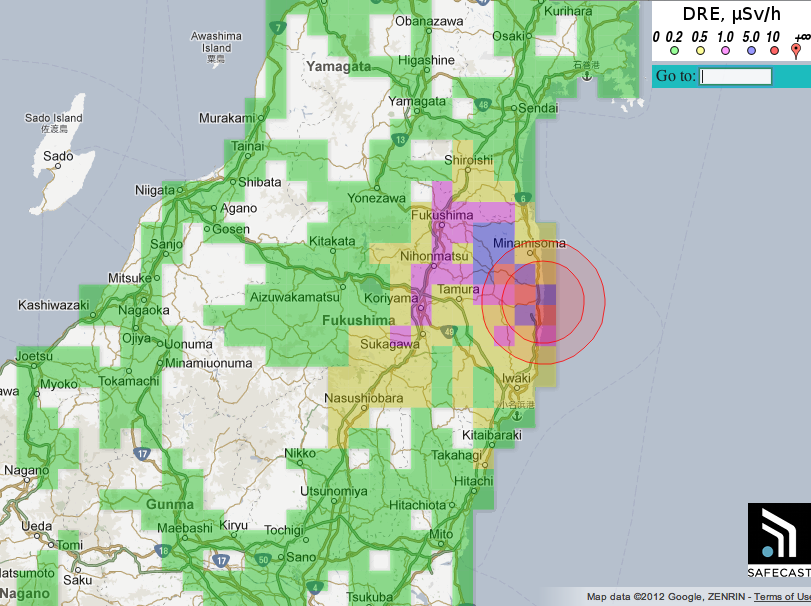
\includegraphics[width=0.3\linewidth]{figures/fusion_map.png}
  %\caption{caption 1}
  \label{fig:subfig1}
}
\subfigure[Individual drive map. Every point correspond to a single
          measurement. We can observe how it is possible to densely
          cover residential areas.]{
  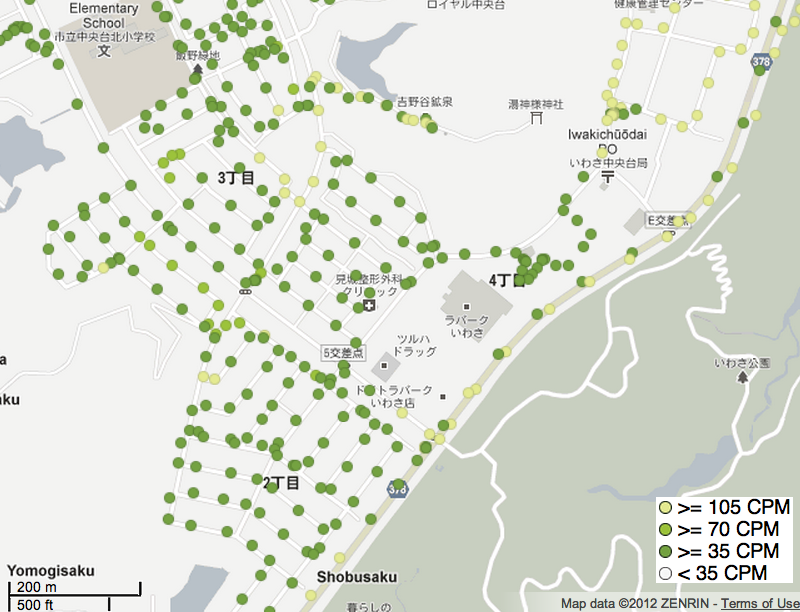
\includegraphics[width=0.3\linewidth]{figures/iwaki_drive.png}
  %\caption{caption 2}
  \label{fig:subfig2}
}
\subfigure[Our sensor fixed on a car. The box contains the Geigier counter
          a microcontroller to count the pulses from the counter, a GPS USB
          dongle and small USB hub. We can see the USB cord that links to
          the netbook in the car.]{
  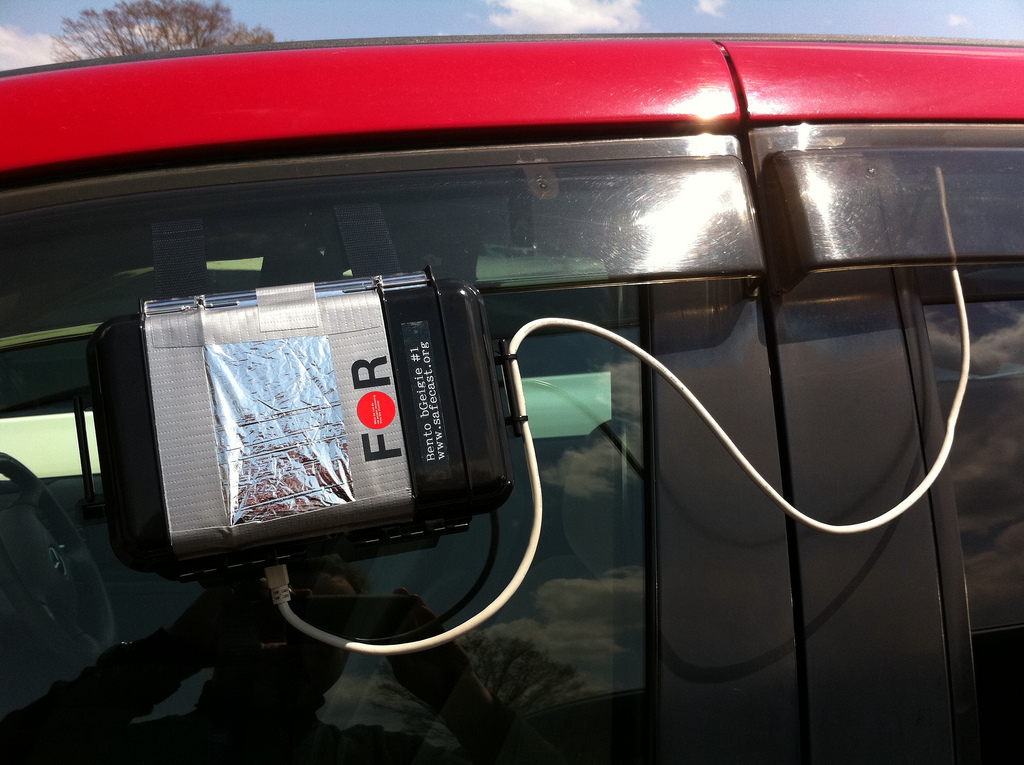
\includegraphics[width=0.3\linewidth]{figures/bgeigie.jpg}
  %\caption{caption 2}
  \label{fig:subfig3}
}
%\label{fig:subfigureExample}
%\caption[Optional caption for list of figures]{Caption of subfigures \subref{fig:subfig1}, \subref{fig:subfig2} and \subref{fig:subfig3}}
\end{figure}

\section*{Acknowledgment}
Keio, Tokyo Hackerspace, ...
%The authors would like to thank...
%more thanks here


% trigger a \newpage just before the given reference
% number - used to balance the columns on the last page
% adjust value as needed - may need to be readjusted if
% the document is modified later
%\IEEEtriggeratref{8}
% The "triggered" command can be changed if desired:
%\IEEEtriggercmd{\enlargethispage{-5in}}

% references section

%% this is required to also have a recap. list of references.
% \printbibliography

% We don't use standard bibliography in this paper
% can use a bibliography generated by BibTeX as a .bbl file
% BibTeX documentation can be easily obtained at:
% http://www.ctan.org/tex-archive/biblio/bibtex/contrib/doc/
% The IEEEtran BibTeX style support page is at:
% http://www.michaelshell.org/tex/ieeetran/bibtex/
% \bibliographystyle{IEEEbib}
% argument is your BibTeX string definitions and bibliography database(s)
% \bibliography{IEEEabrv,bibliography}

% that's all folks
\end{document}


